\documentclass{article}
    % General document formatting
    \usepackage[margin=0.7in]{geometry}
    \usepackage[parfill]{parskip}
    \usepackage[utf8]{inputenc}
    \usepackage{amsmath}
    \usepackage{tikz}
    \usepackage{fancyhdr}
    \usepackage{multicol}

    \usetikzlibrary{positioning}

\pagestyle{fancy}
\fancyhf{}
\rhead{Edgar Jacob Rivera Rios - A01184125}

\begin{document}
\section*{2.3.1 Propositional Logic.}
Prove the following logical equivalences making use of semantic tableaux:
\renewcommand{\labelenumi}{\alph{enumi})}
\begin{enumerate}
    \item $A \wedge (B \vee C) \equiv (A \wedge B) \vee (A \wedge C)$
    \begin{multicols}{2}
        \begin{center}
            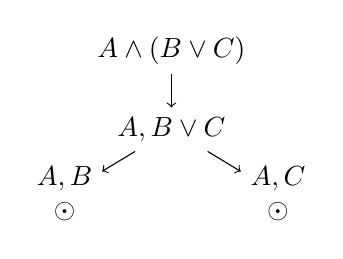
\begin{tikzpicture}[xscale=1.3, yscale=1]
                \node (top) at (0,0) {$A \wedge (B \vee C)$};
                \node [below of = top] (middle)  {$A, B \vee C$};
                \node [below left = 0.1 of middle, align=center] (left)  {$A, B$\\$\odot$};
                \node [below right = 0.1 of middle, align=center] (right)  {$A, C$\\$\odot$};
                \draw [->] (top) edge (middle) (middle) edge (left) (middle) edge (right);
            \end{tikzpicture}
        \end{center}
        \begin{center}
            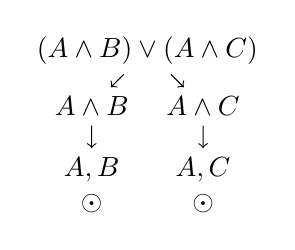
\begin{tikzpicture}[xscale=1.3, yscale=1]
                \node (top) at (0,0) {$(A \wedge B) \vee (A \wedge C)$};
                \node [below left of = top] (left)  {$A \wedge B$};
                \node [below right of = top] (right)  {$A \wedge C$};
                \node [below of = left, align=center] (left2)  {$A, B$\\$\odot$};
                \node [below of = right, align=center] (right2)  {$A, C$\\$\odot$};
                \draw [->] (top) edge (left) edge (right) (left) edge (left2) (right) edge (right2);
            \end{tikzpicture}
        \end{center}
    \end{multicols}

    \item $A \vee B \equiv \neg(\neg A \wedge \neg B)$
    \begin{multicols}{2}
        \begin{center}
            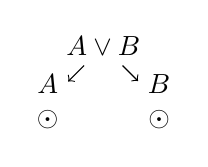
\begin{tikzpicture}[xscale=1.3, yscale=1]
                \node (top) at (0,0) {$A \vee B$};
                \node [below left of = top, align=center] (left) {$A$\\$\odot$};
                \node [below right of = top, align=center] (right) {$B$\\$\odot$};
                \draw [->] (top) edge (left) (top) edge (right);
            \end{tikzpicture}
        \end{center}
        \begin{center}
            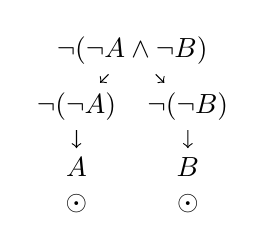
\begin{tikzpicture}[xscale=1.3, yscale=1]
                \node (top) at (0,0) {$\neg(\neg A \wedge \neg B)$};
                \node [below left of = top] (left)  {$\neg(\neg A)$};
                \node [below right of = top] (right)  {$\neg(\neg B)$};
                \node [below of = left, align=center] (left2)  {$A$\\$\odot$};
                \node [below of = right, align=center] (right2)  {$B$\\$\odot$};
                \draw [->] (top) edge (left) edge (right) (left) edge (left2) (right) edge (right2);
            \end{tikzpicture}
        \end{center}
    \end{multicols}

    \item $A \wedge B \equiv \neg(\neg A \vee \neg B)$
    \begin{multicols}{2}
        \begin{center}
            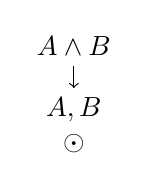
\begin{tikzpicture}[xscale=1.3, yscale=1]
                \node (top) at (0,0) {$A \wedge B$};
                \node [below of = top, align=center] (bottom)  {$A, B$\\$\odot$};
                \draw [->] (top) edge (bottom);
            \end{tikzpicture}
        \end{center}
        \begin{center}
            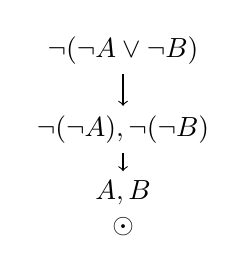
\begin{tikzpicture}[xscale=1.3, yscale=1]
                \node (top) at (0,0) {$\neg(\neg A \vee \neg B)$};
                \node [below of = top] (middle)  {$\neg(\neg A), \neg(\neg B)$};
                \node [below of = middle, align=center] (bottom)  {$A, B$\\$\odot$};
                \draw [->] (top) edge (middle) (middle) edge (bottom);
            \end{tikzpicture}
        \end{center}
    \end{multicols}

    \item $A \rightarrow B \equiv \neg A \vee B$
    \begin{multicols}{2}
        \begin{center}
            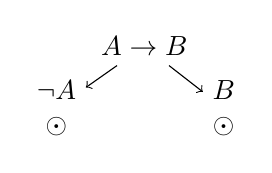
\begin{tikzpicture}[xscale=1.3, yscale=1]
                \node (top) at (0,0) {$A \rightarrow B$};
                \node [below left = 0.1 of top, align=center] (left) {$\neg A$\\$\odot$};
                \node [below right = 0.1 of top, align=center] (right) {$B$\\$\odot$};
                \draw [->] (top) edge (left) (top) edge (right);
            \end{tikzpicture}
        \end{center}
        \begin{center}
            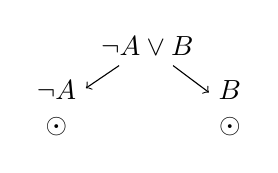
\begin{tikzpicture}[xscale=1.3, yscale=1]
                \node (top) at (0,0) {$\neg A \vee B$};
                \node [below left = 0.1 of top, align=center] (left)  {$\neg A$\\$\odot$};
                \node [below right = 0.1 of top, align=center] (right)  {$B$\\$\odot$};
                \draw [->] (top) edge (left) edge (right);
            \end{tikzpicture}
        \end{center}
    \end{multicols}

    \item $A \rightarrow B \equiv \neg (A \wedge \neg B)$
    \begin{multicols}{2}
        \begin{center}
            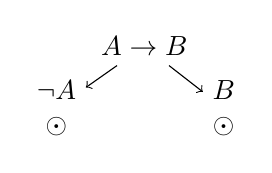
\begin{tikzpicture}[xscale=1.3, yscale=1]
                \node (top) at (0,0) {$A \rightarrow B$};
                \node [below left = 0.1 of top, align=center] (left) {$\neg A$\\$\odot$};
                \node [below right = 0.1 of top, align=center] (right) {$B$\\$\odot$};
                \draw [->] (top) edge (left) (top) edge (right);
            \end{tikzpicture}
        \end{center}
        \begin{center}
            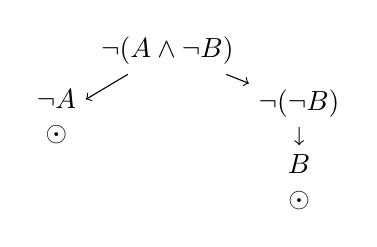
\begin{tikzpicture}[xscale=1.3, yscale=1]
                \node (top) at (0,0) {$ \neg (A \wedge \neg B)$};
                \node [below left = 0.1 of top, align=center] (left)  {$\neg A$\\$\odot$};
                \node [below right = 0.1 of top] (right)  {$\neg(\neg B)$};
                \node [below of = right, align=center] (right2)  {$B$\\$\odot$};
                \draw [->] (top) edge (left) edge (right) (right) edge (right2);
            \end{tikzpicture}
        \end{center}
    \end{multicols}

\end{enumerate}
\newpage

\section*{2.3.2 Propositional Logic.}
Prove or disprove making use of semantic tableaux:
\begin{enumerate}
    \item $\models (A \rightarrow B) \vee (B \rightarrow A)$
    \begin{center}
        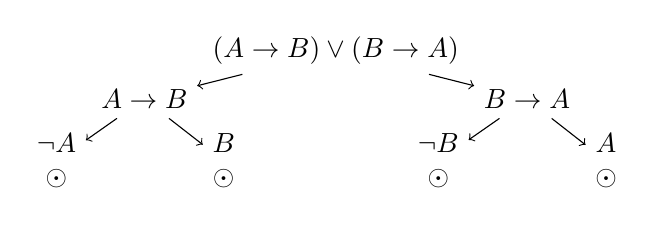
\begin{tikzpicture}[xscale=1.3, yscale=1]
            \node (top) at (0,0) {$(A \rightarrow B) \vee (B \rightarrow A)$};
            \node [below left = 0.1 of top, align=center] (left) {$A \rightarrow B$};
            \node [below right = 0.1 of top, align=center] (right) {$B \rightarrow A$};
            \node [below left = 0.1 of left, align=center] (left1) {$\neg A$\\$\odot$};
            \node [below right = 0.1 of left, align=center] (right1) {$B$\\$\odot$};
            \node [below left = 0.1 of right, align=center] (left2) {$\neg B$\\$\odot$};
            \node [below right = 0.1 of right, align=center] (right2) {$A$\\$\odot$};
            \draw [->] (top) edge (left) (top) edge (right);
            \draw [->] (left) edge (left1) (left) edge (right1);
            \draw [->] (right) edge (left2) (right) edge (right2);
        \end{tikzpicture}
    \end{center}
    As each item is represented only one, we can assume that this is always true

    \item $\models ((A \rightarrow B) \rightarrow B) \rightarrow B$
    \begin{center}
        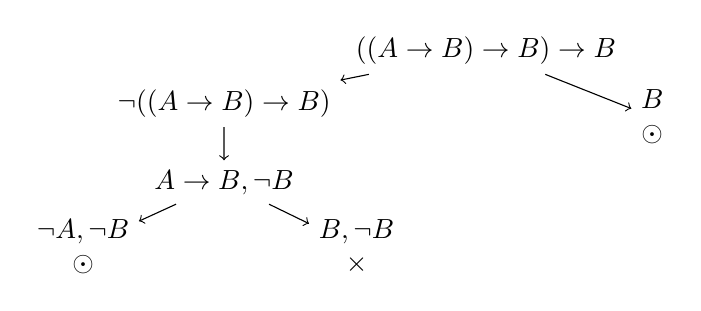
\begin{tikzpicture}[xscale=1.3, yscale=1]
            \node (top) at (0,0) {$((A \rightarrow B) \rightarrow B) \rightarrow B$};
            \node [below left = 0.1 of top, align=center] (left) {$\neg ((A \rightarrow B) \rightarrow B)$};
            \node [below right = 0.1 of top, align=center] (right) {$B$\\$\odot$};
            \node [below of = left, align=center] (left1) {$A \rightarrow B, \neg B$};
            \node [below left = 0.1 of left1, align=center] (left2) {$\neg A, \neg B$\\$\odot$};
            \node [below right = 0.1 of left1, align=center] (right1) {$B, \neg B$\\$\times$};
            \draw [->] (top) edge (left) (top) edge (right);
            \draw [->] (left) edge (left1) (left1) edge (left2) (left1) edge (right1);
        \end{tikzpicture}
    \end{center}
    As we found a contradiction, this is not always true
\end{enumerate}
\end{document}